% !Mode:: "TeX:UTF-8"
\chapter{系统测试评估}

\section{系统测试}
\subsection{测试环境}
测试所用系统环境如下表
\begin{table}
    \centering
    \caption{系统测试环境}
    \label{test-env}
    \begin{tabular}{r|l}
        \hline
        \multirow{2}*{硬件环境} & CPU: Pentium(R) Dual-Core CPU E6600 @ 3.06GHz 3.07GHz \\
                                & 内存: 4.00GB \\ \hline
        \multirow{2}*{软件环境} & 操作系统: Windows 7 64位 \\
                                & 编译器: Microsoft Visual Studio 2010 Ultimate \\
                                & Python: v2.7.3 \\
                                & MeshLab: v1.3.2 \\
                                & ParaView: 4.0.0-RC2 64bit  \\ \hline
    \end{tabular}
\end{table}

\subsection{体素化测试}
测试数据为人体大肠网格模型数据。数据基本信息如表\ref{obj-info}。
\begin{table}
    \centering
    \caption{大肠测试网格数据信息}
    \label{obj-info}
    \begin{tabular}{c|c}
        \hline
        数据大小 & 36,260,461字节 \\ \hline
        顶点数 & 589384 \\ \hline
        面数 & 1178208 \\ \hline
    \end{tabular}
\end{table}

使用体素化转换脚本,测试结果如表\ref{test-voxelization}。
\begin{table}
    \centering
    \caption{大肠测试网格数据体素化测试结果}
    \label{test-voxelization}
    \begin{tabular}{c|c}
        \hline
        生成的体数据信息大小 & 82,102,962字节 \\ \hline
        生成的体数据尺寸 & 474×391×443 \\ \hline
        耗时  & 836.855s (13min56.855s)
    \end{tabular}
\end{table}

耗时比较长,由于体素化本身就是一个十分耗时的工作,并且该脚本没有做任何优化,这个数据在可接受范围内。

使用MeshLab查看原始网格数据、使用ParaView查看生成出来的体数据,在三个坐标轴方向对比结果如图\ref{mesh-vol}。
\begin{figure}[h!]
    \centering
    \begin{tabular}{cc}
        \subfigure[$x$轴方向网格数据]{
            \label{mesh-x}
            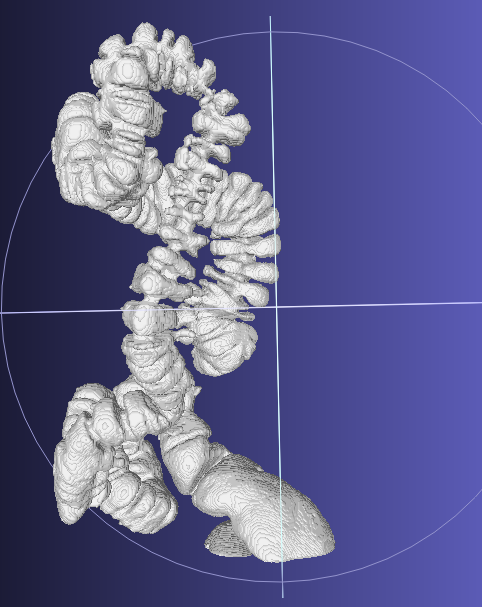
\includegraphics[width=.35\textwidth]{figure/mesh_x.png}
        } \hspace{7em} &
        \subfigure[$x$轴方向体数据]{
            \label{vol-x}
            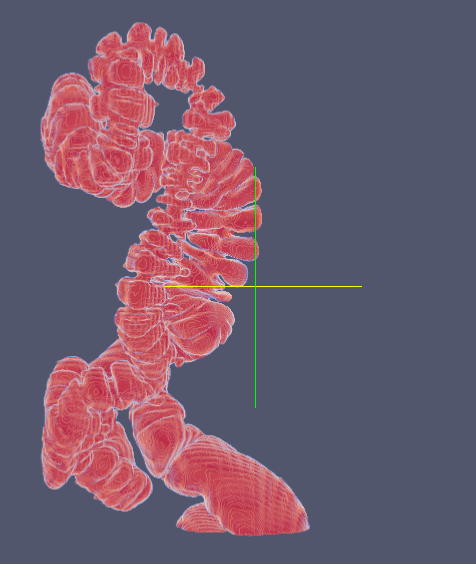
\includegraphics[width=.35\textwidth]{figure/vol_x.png}
        } \\
        
        \subfigure[$y$轴方向网格数据]{
            \label{mesh-y}
            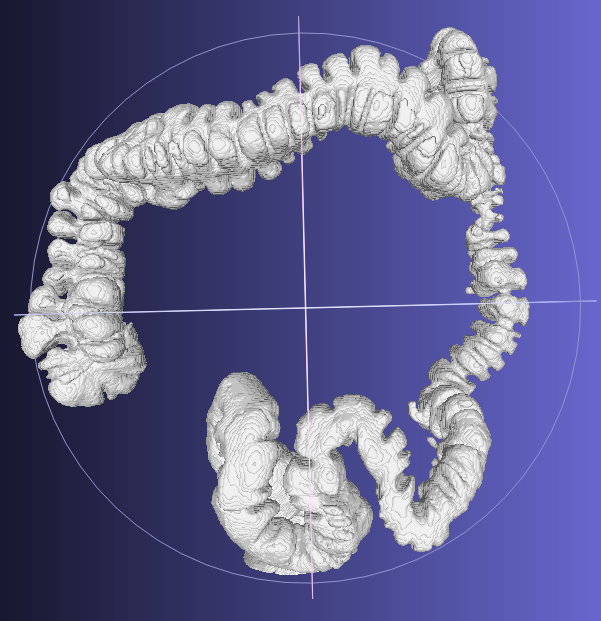
\includegraphics[width=.35\textwidth]{figure/mesh_y.png}
        } \hspace{7em} &
        \subfigure[$y$轴方向体数据]{
            \label{vol-y}
            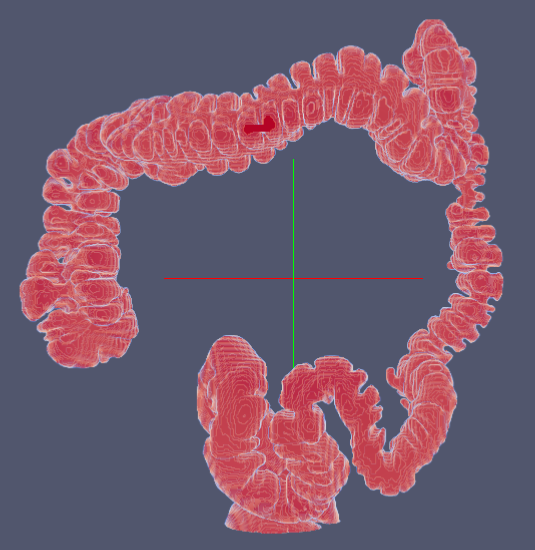
\includegraphics[width=.35\textwidth]{figure/vol_y.png}
        }\\
        
        \subfigure[$z$轴方向网格数据]{
            \label{mesh-z}
            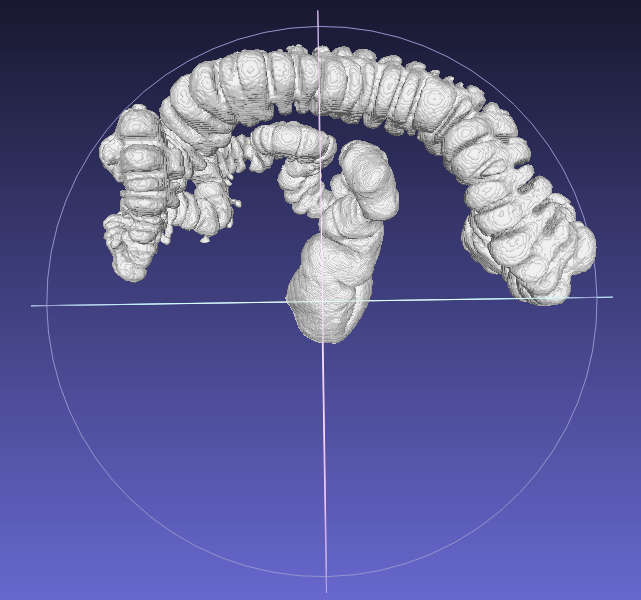
\includegraphics[width=.35\textwidth]{figure/mesh_z.png}
        } \hspace{7em} &
        \subfigure[$z$轴方向体数据]{
            \label{vol-z}
            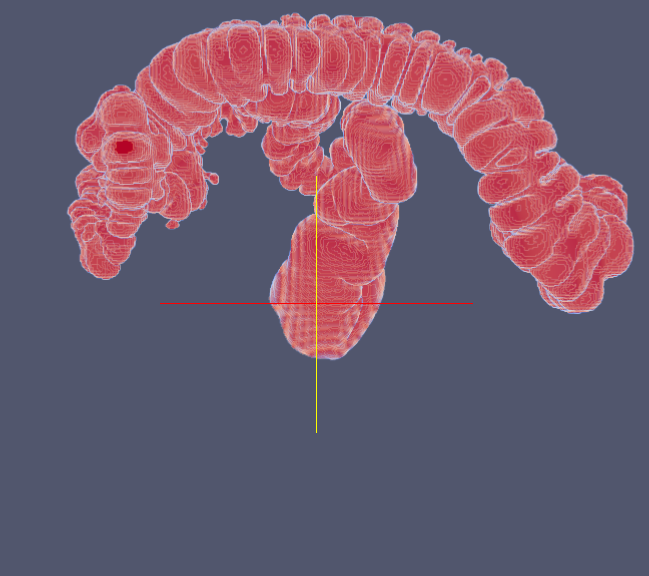
\includegraphics[width=.35\textwidth]{figure/vol_z.png}
        } \\
    \end{tabular}
    \caption{体素化效果图}
    \label{mesh-vol}
\end{figure}
看图可知,转化效果良好,在各个坐标轴方向的图形是完全一致的。

\subsection{3D中心路径提取}
使用上一步生成的数据进行测试,测试时间包括文件读写以及输出的耗时,总耗时平均为93s。生成的结果如下图\ref{test-skel}:
\begin{figure}[h!]
    \centering
    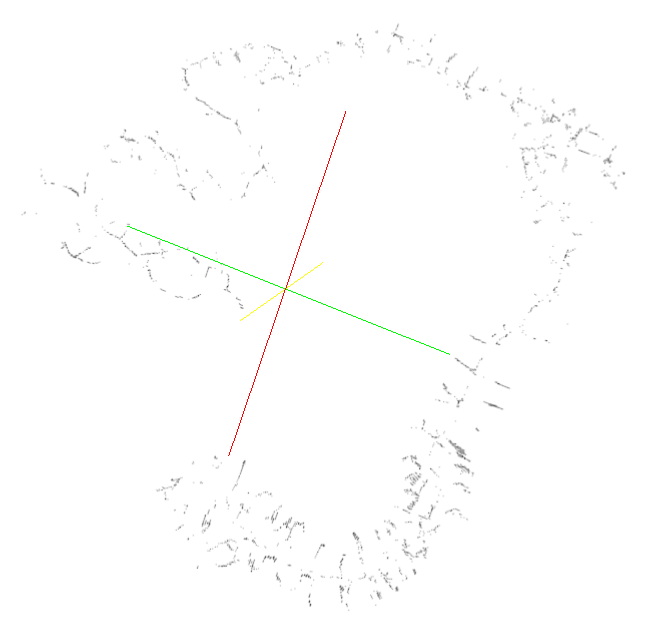
\includegraphics[width=400bp]{figure/skel.png}
    \caption{人体大肠3D中心路径}
    \label{test-skel}
\end{figure}

由于数据分辨率不够高,最终得到的路径存在不连通的情况,这个有待解决。

其他测试数据
\begin{table}
    \centering
    \caption{体数据中心路径提取测试结果}
    \label{test-other}
    \begin{tabular}{c|c|c|c|c}
        \hline
        数据描述 & 立方体      & 圆柱体       & 圆环        & 螺旋 \\ \hline
        尺寸     & 250×250×250 & 250×250×250 & 250×250×250 & 250×250×250 \\ \hline
        平均耗时 & 18s        &  13s         & 11s         & 11s \\ \hline
    \end{tabular}
\end{table}

使用ParaView查看生成的骨架,立方体效果如图\ref{test-other-result-1}所示,其余的图形请查看附录图\ref{test-other-result-2}。
\begin{figure}[h!]
    \centering
    \subfigure[立方体体数据]{
        \label{cuboid_raw}
        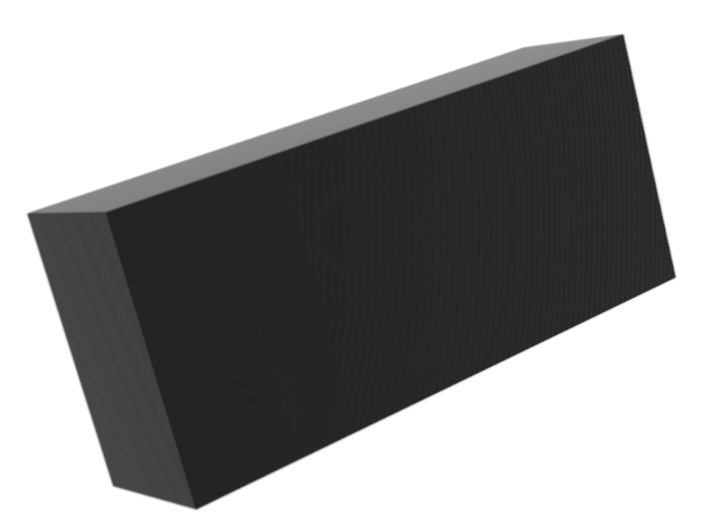
\includegraphics[width=.4\textwidth]{figure/other_test/cuboid_raw.png}
    }
    \hspace{2em} % 水平间隔
    \subfigure[立方体骨架]{
        \label{cuboid_skel}
        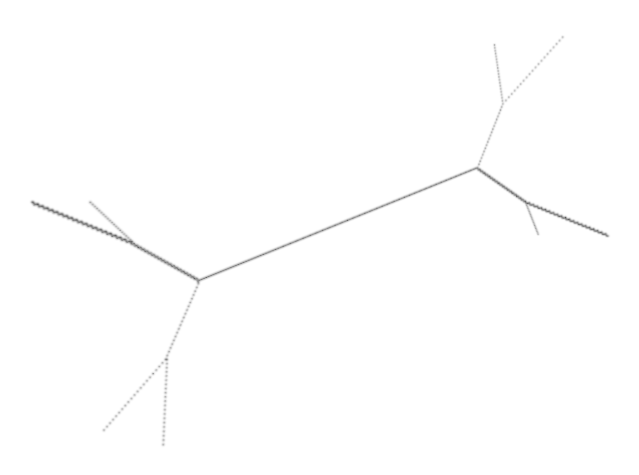
\includegraphics[width=.4\textwidth]{figure/other_test/cuboid_skel.png}
    }
    \caption{立方体体数据中心路径提取效果图}
    \label{test-other-result-1}
\end{figure}

\section{评估}
本模块主要针对3D物体中心路径提取算法进行了研究,并且做了实现。本算法原理简单并且易于实现,算法本身对与用户只暴露一个阈值,对于没有经验的用户体验良好,并且效率较高。在分辨率足够的情况下,能够满足漫游的需求。当然这个算法存在很多不足之处,体素化功能薄弱,对于截面为环形的物体以及分辨率较低的物体不能很好的处理,算法效果受数据影响大,在分辨率较低的情况下,生成的3D中心路径存在不连续的情况。

\section{本章小结}
本章对该模块的核心功能进行了测试,使用了多份测试数据,并做了相应的记录。通过对模块的测试,可以使程序本身更具鲁棒性。
